\chapter{Numerabilità e funzioni}

Questi appunti riguardano le lezioni introduttive sulla numerabilità.


\section{Finito vs. Infinito}

Siamo interessati a questa problematica. Perché? Se avessimo solo da calcolare funzioni di input
finiti con output finiti non avremmo troppe difficoltà. I nostri programmi diventano interessanti
quando andiamo a lavorare su degli input infiniti. Ad esempio, potremmo avere una struttura dati
dinamica come input. Ancora, un programma che lavora su una lista dovrebbe ragionevolmente
funzionare per tutte le liste. I nostri algoritmi dovrebbero essere in grado di accettare una
certa quantità di input infiniti diversi.

L'infinito è anche interessante a livello di complessità computazionale. Nella parte di
complessità computazionale guarderemo al comportamento asintotico del programma al crescere della
dimensione dell'input.

Un'altra problematica interessante è la seguente: a volte l'input stesso dei nostri programmi è
infinito.  Ad esempio, il nostro programma potrebbe essere un automa per un linguaggio libero da
contesto. Il nostro input, un linguaggio, può essere un insieme infinito. 

\begin{figure}[h]
    \centering
    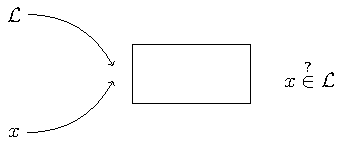
\includegraphics{img/LanguageExample.pdf}
    \caption{Schematizzazione di un automa per un linguaggio $\Lang$}
\end{figure}

Come facciamo a dare al programma un input infinito? L'unico modo è fornire al programma una
descrizione finita dell'input. Creiamo quindi una struttura generativa finita che, da un insieme
finito di oggetti, ci permette di crearne dinamicamente di nuovi.

Questo esempio ci mostra come in questo ambito abbiamo un doppio livello di discussione:
\begin{itemize}

    \item uno descrittivo: a questo livello parlo di quello che mi serve per descrivere ciò di cui
    voglio parlare (e.g. la grammatica per un linguaggio). Vi sono una serie di problematiche legate
    a questo livello: la descrizione che do è giusta? È unica? Ce n'è una canonica? Ad esempio,
    date due grammatiche posso decidere se queste definiscono lo stesso linguaggio?

    \item uno denotazionale: a questo livello parlo veramente del mio oggetto in questione, a
    prescindere da qualsiasi descrizione se ne possa dare (e.g. un linguaggio). Abbiamo le stesse
    problematiche già viste per il livello descrittivo 

\end{itemize}

Il livello descrittivo è anche detto intensionale, quello denotazionale invece estensionale.

Anche per i programmi vale questa distinzione: la funzione calcolata da un programma fa parte del
livello denotazionale. Una funzione è descritta mediante il suo grafo. Non avendo modi diretti,
ovvero finiti, di descrivere la funzione usiamo un programma, che fa parte del livello descrittivo.
Una problematica interessante è la seguente: esiste una maniera di descrivere una funzione che non
mi dia anche un metodo effettivo per calcolarla (non un programma insomma)? 

Siamo costretti ad avere questi due tipi di livelli? Sì se l'oggetto di cui vogliamo parlare è
infinito. La comunicazione presuppone una descrizione finita dell'oggetto infinito.

Tutta la nostra intuizione è basata sul finito. Tuttavia molte cose che non valgono per il finito
valgono per l'infinito. Ad esempio è possibile mettere in corrispondenza biunivoca un sottoinsieme
stretto di un insieme infinito con l'insieme stesso, a differenza del caso finito. Questo è fuori
dalla nostra intuizione immediata degli insiemi.

A volte vogliamo fare ricerche infinite, e.g. su strutture dati infinite. Ad esempio potrei voler
verificare che una stringa $x$ appartenga ad un linguaggio $\Lang$ generando tutte le stringhe da
una grammatica per $\Lang$ e decidere ``Sì'' se $x$ compare. Ho un modo per dire se in una ricerca
troverò quello che cerco? In generale no. Questo problema è fondamentale perché è
frequentissimo. Parleremo in questi casi qui di semi-decisione. Notiamo inoltre che sul
complementare, ovvero $x \notin \Lang$, non possiamo dire niente.

Noi considereremo funzioni da $\Nat$ a $\Nat$ o, al massimo, da $\Nat^{k}$ a $\Nat$. Questo perché
i numeri naturali sono la più semplice struttura infinita. Questo non ci pone limitazioni di alcun
tipo. Se noi siamo interessati ad aspetti di calcolabilità tutto è alla fine riconducibile ad un
numero binario. Questa traduzione da un oggetto qualsiasi ad un numero naturale prende il nome di
Gödelizzazione. Ai tempi ($\sim 1930$) fu un'idea rivoluzionaria, ma dal punto di vista di un informatico
dovrebbe sembrare più naturale.

\section{Numerabilità}

Le seguenti sono note alle slide

\begin{defn}
    Un insieme $A$ si dice numerabile se esiste una funzione suriettiva $f$ dall'insieme
    dei numeri naturali $\Nat$ in $A$. $f$ è detta funzione di enumerazione.
\end{defn}

Un esempio di insieme numerabile è $\Nat$. Inoltre ogni sottoinsieme di un insieme numerabile è
ancora numerabile. La funzione $f$ ci dà anche un metodo di enumerazione degli elementi del
codominio di $f$.

\begin{lem}
   Sia $A$ numerabile. Allora $\set{*} \oplus A$ è ancora numerabile.
\end{lem}
\begin{proof}
    Sia $f : \Nat \to A$ la funzione di enumerazione di $A$. definiamo $g : \Nat \to \set{*} \oplus A$
    nel modo seguente:
    \begin{equation*}
        g(x) =
        \begin{cases}
            \case{g(0)=*}{}\\
            \case{g(x+1)=f(x)}{}\\
        \end{cases}
    \end{equation*}
    Chiaramente $g$ è suriettiva.
\end{proof}

Aggiungere un elemento non intacca la numerabilità di un insieme. Basta uno shift per avere una
nuova enumerazione di $A$. La numerabilità è resistente all'operazione di estensione.
\begin{cor}
    Sia $A$ numerabile e $D$ finito. Allora $D \oplus A$ è ancora numerabile.
\end{cor}

\begin{lem}
    L'unione di due insiemi numerabili $A$ e $B$ è ancora numerabile.
\end{lem}
\begin{proof}
    Siano $f$ e $g$ le due funzioni di enumerazione di $A$ e $B$. $A \oplus B$ è allora enumerato dalla seguente
    funzione $h$:
    \begin{equation*}
        h(x) =
        \begin{cases}
            \case{h(2x)=f(x)}{}\\
            \case{h(2x+1)=g(x)}{}\\
        \end{cases}
    \end{equation*}
\end{proof}

\begin{cor}
    Un unione finita di insiemi numerabili è numerabile.
\end{cor}
\begin{cor}
    Se $D$ è finito e $A$ è numerabile allora $D \times A$ è numerabile.
\end{cor}
\begin{proof}
    Per $A,B$ numerabili abbiamo $A \oplus B$ numerabile. Prendiamo in considerazione l'unione
    disgiunta di A con se stesso $k$ volte:
    \begin{equation*}
        \overbrace{\underset{0}{A} \oplus \underset{1}{A} \oplus \cdots \oplus
        \underset{k}{A}}^{\text{$k$ volte}}
    \end{equation*}
    Questo insieme è chiaramente numerabile. Chiamiamolo $A_{k}$. Abbiamo che:
    \begin{equation*}
        A_{k} = \bigcup_{i=0}^{k-1}\set{<i,a> \mid a \in A} = \set{<i,a> \mid a \in A, i \in
        \set{0,\dotsc,k-1}} = A \times K
    \end{equation*}
    da cui l'asserto.
\end{proof}

Possiamo enumerare $\Nat \times \Nat$? Vediamo com'è fatto questo insieme. Avremo $(0,0), (0,1),
(0,2),\dotsc$, dopodiché, sulla prossima riga, avremo $(1,0), (1,1), (1,2),\dotsc$, e così via
all'infinito. Il modo più conveniente per visualizzarlo è pensare a dei punti nel piano. 

Possiamo enumerarli? Sarebbe sbagliato numerare per righe o per colonne. Questo perché le righe e
le colonne sono infinite, iterando su una riga non passerò mai alla prossima. Che tecnica usiamo?
Dove tailing. Numeriamo per diagonali. Ce ne sono altre di numerazioni possibili. Va bene qualsiasi
``gioco dell'oca'' che passa per ogni coppia una e una sola volta.

\begin{figure}[h]
    \centering
    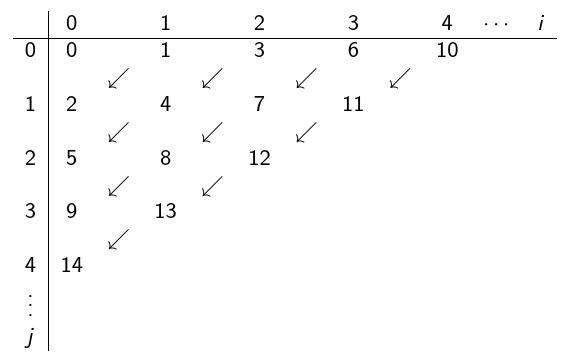
\includegraphics[scale=0.5]{img/DoveTailing.jpg}
    \caption{Dove tailing}
\end{figure}

Questa codifica si ottiene nel seguente modo:
\begin{equation*}
    <i,j> = j + \sum_{k=0}^{i+j}k = \frac{(i+j)^{2}+i+3j}{2}
\end{equation*}
ed è giustificata dal ragionamento seguente: la somma delle componenti $i$ ed $j$ per i punti su di una
stessa diagonale è costante e pari al numero di diagonali già interamente percorse. Il numero di
punti del piano già visitati in queste diagonali è
\begin{equation*}
    \sum_{k=0}^{i+j}k = \frac{(i+j)(i+j+1)}{2}
\end{equation*}
Per visitare l'elemento $<i,j>$ dovrò ancora percorrere $j$ passi lungo l'ultima diagonale, da cui
la formula precedente.

Importante: Il dove tailing non è la diagonalizzazione.

Come corollario abbiamo che il prodotto cartesiano di due insiemi numerabili è numerabile.

È facile dimostrare che posso avere delle biezioni tra $\Nat^{k}$ e $\Nat$, in modo da codificare
delle tuple di numeri con un numero solo. In altre parole c'è una procedura algoritmica che mi
permette di passare da una tupla al corrispondente numero $n$ e da $n$ alla corrispondente tupla. Di
conseguenza $\Nat^{k}$, per $k$ naturale, è ancora numerabile.

\begin{lem}
    L'unione di un insieme numerabile di insiemi numerabili è ancora numerabile.
\end{lem}
\begin{proof}
    Sia $A$ un insieme numerabile e sia $f$ la sua funzione di enumerazione. Sia $\set{B_{a}\mid a
    \in A}$ una collezione di insiemi numerabili, ciascuno enumerato da una funzione $g_{a}$. La funzione
    $h : \Nat \times \Nat \to \bigcup_{a \in A}B_{a}$ definita da
    \begin{equation*}
        h(n,m) = g_{f(n)}(m)
    \end{equation*}
    è suriettiva.
\end{proof}

\begin{lem}
    Se $A$ è un insieme numerabile, anche $\bigcup_{i \in \Nat} A^{i}$ è numerabile.
\end{lem}

Consideriamo l'operatore di Kleene sull'alfabeto $\Sigma$: $\Sigma^{*}$. Anche questo insieme è
numerabile, perché è l'unione numerabile di insiemi numerabili (ricordiamo che $A^{k}$ è numerabile).

Un altro insieme numerabile interessante è l'insieme delle parti finite:
\begin{equation*}
    \Parts_{\textit{fin}}(\Nat) = \{A \mid A \subseteq \Nat, \textit{$A$  è finito}\}
\end{equation*}

Abbiamo due piani di infinità nei programmi: l'infinità dell'input e l'infinità del tempo di
calcolo, in quanto il mio programma può divergere su un dato input.

L'insieme di funzioni da $A$ a $B$ ha cardinalità $B^{A}$.

Possiamo caratterizzare l'insieme delle coppie su $A$, $A \times A = A^{2}$, come una funzione
dall'insieme $\BOOL = \{0,1\}$ all'insieme $A$. $f(x)$ può essere così definita: data
una coppia $<a_{1},a_{2}>$, $f(x)$: $ x \mapsto $ if $x$ then $a_{1}$ else $a_{2}$. Al posto dei booleani potremmo
avere un qualsiasi insieme di cardinalità 2.

$A^{K}$ è isomorfo all'insieme delle funzioni $f: K \to A$.

La funzione è utile sia come strumento di calcolo che come strumento di codifica dei dati.

Lo spazio delle funzioni da un insieme finito ad un insieme numerabile è ancora numerabile.

\section{Diagonalizzazione}

Consideriamo lo spazio delle funzioni da un insieme numerabile ad un altro insieme numerabile.
Ancora più semplicemente, possiamo considerare le funzioni da $\Nat$ a 2 (o $\BOOL$).

L'insieme delle funzioni da $A$ a $\BOOL$ è isomorfo all'insieme delle parti di $A$.

Per denotare un sottoinsieme si può dare una funzione caratteristica, che restituisce 1 se un
elemento fa parte del sottoinsieme e 0 altrimenti.

\begin{thm}
    Per ogni insieme $A$ non esiste una funzione suriettiva da $A$ in $\Parts(A)$.
\end{thm}
\begin{proof}
    Sia $f : A \to \Parts(A)$ una funzione suriettiva da $A$ all'insieme delle parti di $A$. Data
    $f$ posso costruire parametricamnente $\Delta_{f}$ così fatto:
    \begin{equation*}
        \Delta_{f} = \{a \mid a \in A, a \notin f(a)\}
    \end{equation*}
    Essendo $f$ suriettiva esiste $a$ tale che $f(a) = \Delta_{f}$. Ci chiediamo ora, $a \in f(a)$?
    \begin{equation*}
        a \in f(a) \iff a \in \Delta_{f} \iff a \in A \land a \notin f(a)
    \end{equation*}
    Ma questo è assurdo.
\end{proof}

La tecnica con cui si dimostra questo teorema è detta tecnica diagonale, o diagonalizzazione.
Un'idea intuitiva che giustifica il nome è la seguente: consideriamo una tabella indicizzata per
colonne dagli $a \in A$ e sulle righe dagli $f(a)$ per ogni $a \in A$. Nella cella $(i,j)$ della
tabella avrò 1 se $a_{j} \in f(a_{i})$ e 0 altrimenti. Abbiamo per ogni riga la funzione
caratteristica di $f(a)$, per ogni $a \in A$. Abbiamo ora che la funzione caratteristica di
$\Delta_{f}$ è costruita andando sulla diagonale e prendendo l'elemento $j$ in $\Delta$ se in
corrispondenza sulla diagonale, ovvero alla riga $i$, ho 0, lasciandolo fuori altrimenti. Di
conseguenza la funzione caratteristica che vado a costruire per definire $\Delta$ è diversa da
tutte le funzioni caratteristiche sulle righe almeno per un elemento.

La diagonalizzazione è un metodo semplice per creare un nuovo elemento diverso da tutti quelli di
una lista sotto certe ipotesi.

Dimostriamo che i numeri nell'intervallo $[0,1[$ sono una quantità non numerabile. Come possiamo
descrivere i numeri reali? Possiamo farlo, ad esempio, con la loro rappresentazione decimale: una
infinita successione delle cifre del numero, per ogni numero.

Supponiamo di avere una enumerazione dei numeri reali $r_{0}, r_{1}, r_{2}, \dotsc$. Disegnamo una
tabella con le righe indicizzate dai numeri reali nell'ordine dato dall'enumerazione e con le
colonne indicizzate dai numeri naturali. Per ogni numero della enumerazione possiamo scrivere, in
corrispondenza della colonna $j$, la sua cifra $j$, in ordine da sinistra verso destra. 

Consideriamo la diagonale della tabella. Consideriamo il mapping che per gli elementi dell'insieme
$\{0,\dotsc,4\}$ restituisce 7 mentre per gli elementi dell'insieme $\{5,\dotsc,9\}$ restituisce 3.
Se prendiamo la diagonale e alle sue cifre applichiamo il mapping creato otteniamo un numero che è
diverso da tutti gli elementi dell'enumerazione almeno per la cifra sulla diagonale. Di conseguenza
non fa parte dell'enumerazione. Ma questo è assurdo, dato che avevo supposto di poter enumerare
tutti i numeri reali dell'intervallo $[0,1[$.

Le funzioni da $\Nat$ a 2, a $\{0,\dotsc,9\}$, a $\Nat$ hanno la stessa cardinalità, quella del
continuo, che non è numerabile.

Esistono quindi numeri reali per i quali non esiste una maniera per descriverli.

\section{Definibilità vs. Calcolabilità}

Le funzioni da $\Nat$ a $\Nat$ di cui possiamo parlare hanno cardinalità numerabile. Anche i programmi sono
una quantità numerabile.

Non è però questo il problema che vogliamo affrontare. È evidente per ragioni di cardinalità che
ci sono funzioni che non potremo calcolare. Il problema a cui siamo interessati è: tutte le
funzioni che possiamo definire sono calcolabili o ci sono funzioni definibili ma non calcolabili?

Abbiamo inizialmente il problema di cosa significa definibile. La nozione di definibilità dipende
dal contesto e dal potere espressivo del linguaggio che uso (e.g. linguaggio dell'aritmetica, linguaggio
del secondo ordine, ecc.).

Possiamo formalizzare la nozione di definibilità? No. È possibile dimostrare che l'idea di
definibilità non è definibile. Non è possibile dire quando una cosa è ben definita.

Supponiamo di avere un criterio che scansiona le stringhe e decide se una è una buona definizione o
no. Possiamo quindi definire una sequenza di funzioni e quindi dare una numerazione delle funzioni
definibili. Si può dimostrare che questa definizione di definibilità è incompleta, non cattura
bene il nostro senso intuitivo di definibilità. 

Intuitivamente, possiamo creare una tabella con le righe indicizzate dalle funzioni definite e per
colonne dai numeri naturali. La casella $(i,j)$ contiene il risultato della funzione $f_i$ sul
numero $j$. Supponiamo inoltre di avere funzioni binarie, ovvero che restituiscono 1 o 0. Questa
semplificazione non fa perdere di generalità. 

Con un procedimento diagonale possiamo definire una nuova funzione che non sta nell'enumerazione. Ad
esempio, sia $f(n) = 1 - d_{n}(n)$. Se questa definizione intuitivamente valida non è presente
nell'enumerazione allora il mio criterio è incompleto.  Supponiamo che nella mia enumerazione la
mia funzione $f$ compaia in posizione $m$. Allora avremmo $d_m(m) = f(m) = 1 - d_m(m)$. Ma questo è
assurdo.

Se fissiamo un linguaggio l'insieme delle funzioni definite su quel linguaggio è numerabile. Esiste
quindi una funzione, per quel linguaggio, che mi dica se una definizione è valida. Questa funzione,
tuttavia, non è calcolabile.

\subsection{Paradosso di Russel}

Questo è un vero paradosso, che mise in crisi la matematica agli inizi del XX secolo.

Possiamo pensare ad un insieme come ad una collezione di cose che rispetta certe proprietà. Data
una proprietà $P(x)$ possiamo costruire un insieme che la rispetti:
\begin{equation*}
    \frac{P(t)}{t \in \{x \mid P(x)\}} % the proving package may be useful here
\end{equation*}
Vale anche l'implicazione inversa

Pensiamo alla proprietà $P(x) = ``x \notin x''$. Possiamo costruire l'insieme $U = \{x \mid x \notin x\}$. Ci
chiediamo ora: $U \in U$? Abbiamo che $U \in U \iff U \notin U$. Ma questo è paradossale.

Il problema è che all'inizio del secolo si era tentato di basare la teoria insiemistica sul
principio di comprensione. Per quanto comodo e bello questo, nella forma che abbiamo visto, è causa
di paradossi. Dobbiamo rinunciare all'idea che basti pensare ad una proprietà per poter creare un
insieme che la rispetti.

\subsection{Paradosso di Berry}

%Berry era un bibiliotecario che si era appassionato un pò di matematica. // curiosità storiche
C'è un principio importante nei numeri naturali che dice che dato un sottoinsieme finito dei numeri
naturali esiste un elemento dei naturali che è il più piccolo numero naturale che non appartiene a
questo sottoinsieme.

Supponiamo di definire i numeri con stringhe di lunghezza $d$. Abbiamo quindi un insieme di numeri
che posso definire con al più $d$ caratteri. Possiamo definire $n_d$ come il più piccolo numero
non definibile con meno di $d$ caratteri, e sappiamo che esiste per il principio precedentemente
riportato.

Prendiamo ad esempio $d=100$. Abbiamo che $n_{100}$ non è definibile con meno di 100 caratteri. Eppure
è definito dalla stringa: ``$n_{100}$ non è definibile con meno di 100 caratteri'', che ha meno di 100
caratteri. Questo è assurdo.

%Più formalmente, supponiamo che la definizione sia data dalla stringa $s$ e prendiamo $d_{s} = |s|$.
%$n_{d_{s}}$ è il più piccolo numero non definibile con meno di $d_{s}$ caratteri. Ma $n_{d_{s}}$ è
%definito da $s$. Assurdo. // Non mi sembra corretta

Ci sono paradossi e paradossi. Alcune sono cose che sembrano strane ma in realtà non lo sono così
tanto. Altri sono proprio cattivi, mettono in questione aspetti fondamentali della nostra
intuizione.

Dove sta il problema del paradosso di Berry? Nella stringa $s$, perché la nozione di definibilità non
è definibile, ed $s$ la usa. La definizione data non è una buona definizione.

Ci chiediamo: data una enumerazione $\theta$ delle sentenze dell'aritmetica è possibile generare una
formula che mi dice il valore di verità di una sentenza dell'enumerazione?

Ad ogni sentenza dell'enumerazione associamo un numero, detto di Gödel. Questo perché non possiamo
parlare delle sentenze in sè in aritmetica, ma possiamo parlare solo di numeri. Quindi ci serve un
numero per parlare della sentenza.

La verità è intesa sul modello dei numeri naturali.

Vogliamo una formula \textit{Vera} tale che
\begin{equation*}
    \StdNat \models A \iff \StdNat \models \textit{Vera}(g(A))
\end{equation*}
dove $g(A)$ rappresenta il numero di Gödel di $A$.

Per i numeri naturali c'è un lemma detto lemma di diagonalizzazioe. Questo dice che dato un
predicato è sempre possibile trovare una formula $S$ tale che $\StdNat \models S \iff \StdNat \models
P(g(S))$. È possibile, per una sentenza, dire "quel predicato P vale per me". La dimostrazione è
interessante perché costruttiva.

Prendiamo come $P(x)$ la formula $\lnot \textit{Vero}(x): \StdNat \models P(x) \iff \StdNat \models
\lnot \textit{Vero}(x)$. Possiamo allora costruire $S$ tale che $\StdNat \models S \iff \StdNat
\models \lnot Vero (S)$. Avremmo quindi $\StdNat \models S \iff \StdNat \models \lnot S$. Ma questo è
paradossale.  Quindi non è definibile, nel linguaggio dell'aritmetica, una formula che, data una
sentenza dell'aritmetica, mi dice se questa è vera, in senso aritmetico. Questo risultato è
soprendentemente forte e va sotto il nome di teorema di Tarski.

Un'idea simile viene usata nel teorema di Gödel non con la nozione di verità matematica ma con la
nozione di dimostrabilità. Il risultato è che la formula che afferma la propria indimostrabilità
non è dimostrabile. Da ciò il sistema logico è incompleto, ovvero c'è una formula indimostrabile.
